\documentclass[aps,prd,%showpacs,preprintnumbers,twelvepoint
 ]{revtex4}
\usepackage{graphicx}
\usepackage{color}
\usepackage{slashed}
\usepackage{amsmath}
\usepackage{hyperref}

\newcommand\ppbar{\langle\overline\psi\psi\rangle}
\newcommand{\calM}{{\cal {M}}}
\newcommand{\diag}{{\rm {diag}}}

\begin{document}

\title{Notes on Nuclear PDFs}
\author{Ankita\ \surname{Budhraja}}
\email{ankita@theory.tifr.res.in}
\affiliation{Department of Theoretical Physics, Tata Institute of Fundamental
         Research,\\ Homi Bhabha Road, Mumbai 400005, India.}
\author{Sourendu\ \surname{Gupta}}
\email{sgupta@theory.tifr.res.in}
\affiliation{Department of Theoretical Physics, Tata Institute of Fundamental
         Research,\\ Homi Bhabha Road, Mumbai 400005, India.}
\author{Rishi\ \surname{Sharma}}
\email{rishi@theory.tifr.res.in}
\affiliation{Department of Theoretical Physics, Tata Institute of Fundamental
         Research,\\ Homi Bhabha Road, Mumbai 400005, India.}

\begin{abstract}
Some notes on the nuclear PDFs.
\end{abstract}
\maketitle

\section{Introduction}
One of the effects that need to be included in the calculation of $R_{AA}$ is
that the parton distribution functions (PDFs) in Pb are different from that in
the proton.

There are various parameterizations of this effect fitted to data. Two popular 
ones that are available in tabulated form are
\begin{enumerate}
\item{Results from Ref.~\cite{Eskola:2009uj}. (See Ref.~\cite{Paukkunen:2014pha}
and Ref.~\cite{Eskola:2020yfa} for some more recent papers from the same
group.)}
\item{Results from Ref.~\cite{Kovarik:2015cma}. (See
Ref.~\cite{Schienbein:2009kk} for the first paper from this group.)}
\end{enumerate}

\section{Kinematics}
To set up the kinematics, we consider a collision in the center of mass
coordinates of two protons (or a proton and a neutron). The energy momentum
components of the protons are
\begin{eqnarray}
p_1 &=& (\sqrt{s}/2,0,0,\sqrt{s/4-m_N^2}) \\
&\approx&  (\sqrt{s}/2,0,0,\sqrt{s}/2)\\
p_2 &=& (\sqrt{s}/2,0,0,-\sqrt{s/4-m_N^2}) \\
&\approx&  (\sqrt{s}/2,0,0,-\sqrt{s}/2)
\end{eqnarray}
In our calculations $\sqrt{s}=5.02$TeV. 

Partons from the nucleons (at LHC energies we can assume that the two partons
are gluons) carry fractions $x_a$ and $x_b$ of $p_1$ and $p_2$,
\begin{eqnarray}
p_a &=& x_a p_1 \\
p_b &=&  x_b p_2 \;.
\end{eqnarray}

In the final state, two jets with mass $m_J$, transverse momenta $p_T$,
and transverse mass $m_T=\sqrt{p_T^2+m_J^2}$ are created. Let us assume that
the rapidity of one of the jets is $y$. Then, emergy momentum conservation
gives,
\begin{equation}
x_b = 
  \frac{1}{\sqrt{s}}
  \frac{x_am_T\sqrt{s}\exp(-y) - m_J^2}{x_a\sqrt{s} - m_T\exp(y)}\;.
\end{equation}
(This must be a well known expression since 1960's but I don't have a well
defined reference. For now I'm referring to Ref.~\cite{Sharma:2012dy}.)

We are particularly interested in small angle jets so that $m_J \sim p_T
\Delta\theta \ll p_T$ at central rapidity. For these kinematics,
\begin{equation}
x_b = \frac{p_T x_a}{-p_T + \sqrt{s} x_a}\;.
\end{equation}

For the estimate of a typical hard collision, $x_b\sim x_a$ which gives the
well known estimate of the dominant $x$,
\begin{equation}
x_a \approx \frac{2 p_T}{\sqrt{s}}~\;.\label{eq:xestimate}
\end{equation}

Finally, when we calculate the parton distribution functions (gluonic), then it
is a function of $x$ ad well as the energy scale. We take the relevant energy scale to
be $p_T$.

\begin{equation}
R_{\rm{gPb}}(p_T) = \frac{\phi_g^{\rm{Pb}}(x=\frac{2p_T}{\sqrt{s}}, Q=p_T)}
{\phi_g^{\rm{p}}(x=\frac{2p_T}{\sqrt{s}}, Q=p_T)}\;. \label{eq:RgPb}
\end{equation}

\section{EPS09}
Ref.~\cite{Eskola:2009uj} describes the fitting of 
\begin{equation}
R_{\rm{g/q N}}(x, Q) = \frac{\phi_g^{\rm{Pb}}(x, Q)} {\phi_g^{\rm{p}}(x, Q)}
\end{equation}
for partons $g$ and $q$ for various nuclei $N$. 

The fitted forms are available in tabulated form at
[https://www.jyu.fi/science/en/physics/research/highenergy/urhic/npdfs/eps09]
and are saved in the subdirectory ``EPS09''.  The quantity of interest
$R_{\rm{gPb}}(p_T)$ is calculated using ``EPS09modified.f''.

The results from the program are stored in ``RgPbEPS09.dat'' along with the
errors.

\section{CTEQ15}
Ref.~\cite{Kovarik:2015cma} describes the fitting of 
\begin{equation}
\phi_{g/q}^{\rm{Pb}}(x, Q)
\end{equation}
for partons $g$ and $q$ for various nuclei and for protons and
the ratio $R_{\rm{gPb}}(p_T)$ can be computed easily using Eq.~\ref{eq:RgPb}. 

The fitted forms are available in tabulated form at
[https://ncteq.hepforge.org/]and are saved in the subdirectory ``EPS09''.  The
quantity of interest $R_{\rm{gPb}}(p_T)$ is calculated using
``CalculateRgCTEQ.nb''. The results are stored in ``RgmidvspTCTEQ.dat'',
``RgdownvspTCTEQ.dat'', and ``RgupvspTCTEQ.dat''.


\section{Results}
\begin{figure}[!htbp]
	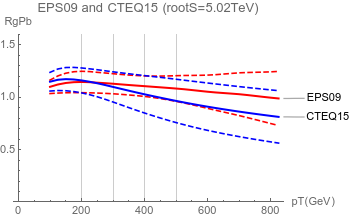
\includegraphics[scale=0.99]{EPS09CTEQ15RgPb.png}
	\caption{Ratio of Nuclear PDFs of Pb-208 and proton as a function of $p_T$.
    $x=\frac{2p_T}{\sqrt{S}}$ (Eq.~\ref{eq:xestimate}) and the scale of the PDFs is taken
    to be $p_T$.}
	\label{fig:RpPb}
\end{figure}

The results above are read using ``EPS09CTEQ15Read.nb'' and plotted in
Fig.~\ref{fig:RpPb}.  In Fig.~\ref{fig:RpPb} we show the ratio of the gluonic
distribution functions in p and in Pb (Eq.~\ref{eq:RgPb}). 

We note that this ratio is slightly larger than $1$ for $p_T\sim 200$GeV. For
larger $p_T$ the error bars are quite large but the results are consistent with
$R_{\rm{gPb}}$ is consistent with being constant or slightly decreasing in this 
regime. 

These results are consistent with
Refs.~\cite{Chatrchyan:2014hqa,Epple:2017qtk}. 
\begin{thebibliography}{9}
%\cite{Eskola:2009uj}
\bibitem{Eskola:2009uj}
K.~J.~Eskola, H.~Paukkunen and C.~A.~Salgado,
%``EPS09: A New Generation of NLO and LO Nuclear Parton Distribution Functions,''
JHEP \textbf{04} (2009), 065
doi:10.1088/1126-6708/2009/04/065
[arXiv:0902.4154 [hep-ph]].
%1103 citations counted in INSPIRE as of 04 Jun 2021

%\cite{Paukkunen:2014pha}
\bibitem{Paukkunen:2014pha}
H.~Paukkunen, K.~J.~Eskola and C.~Salgado,
%``Dijets in p + Pb collisions and their quantitative constraints for nuclear PDFs,''
Nucl. Phys. A \textbf{931} (2014), 331-336
doi:10.1016/j.nuclphysa.2014.07.012
[arXiv:1408.4563 [hep-ph]].
%14 citations counted in INSPIRE as of 04 Jun 2021

%\cite{Eskola:2020yfa}
\bibitem{Eskola:2020yfa}
K.~J.~Eskola, I.~Helenius, P.~Paakkinen and H.~Paukkunen,
%``Impact of dijet and D-meson data from 5.02 TeV p+Pb collisions on nuclear PDFs,''
Nucl. Phys. A \textbf{1005} (2021), 121944
doi:10.1016/j.nuclphysa.2020.121944
[arXiv:2001.10385 [hep-ph]].
%2 citations counted in INSPIRE as of 04 Jun 2021

%\cite{Kovarik:2015cma}
\bibitem{Kovarik:2015cma}
K.~Kovarik, A.~Kusina, T.~Jezo, D.~B.~Clark, C.~Keppel, F.~Lyonnet, J.~G.~Morfin, F.~I.~Olness, J.~F.~Owens and I.~Schienbein, \textit{et al.}
%``nCTEQ15 - Global analysis of nuclear parton distributions with uncertainties in the CTEQ framework,''
Phys. Rev. D \textbf{93} (2016) no.8, 085037
doi:10.1103/PhysRevD.93.085037
[arXiv:1509.00792 [hep-ph]].
%350 citations counted in INSPIRE as of 04 Jun 2021

%\cite{Schienbein:2009kk}
\bibitem{Schienbein:2009kk}
I.~Schienbein, J.~Y.~Yu, K.~Kovarik, C.~Keppel, J.~G.~Morfin, F.~Olness and J.~F.~Owens,
%``PDF Nuclear Corrections for Charged and Neutral Current Processes,''
Phys. Rev. D \textbf{80} (2009), 094004
doi:10.1103/PhysRevD.80.094004
[arXiv:0907.2357 [hep-ph]].
%134 citations counted in INSPIRE as of 04 Jun 2021

%\cite{Sharma:2012dy}
\bibitem{Sharma:2012dy}
R.~Sharma and I.~Vitev,
%``High transverse momentum quarkonium production and dissociation in heavy ion collisions,''
Phys. Rev. C \textbf{87} (2013) no.4, 044905
doi:10.1103/PhysRevC.87.044905
[arXiv:1203.0329 [hep-ph]].
%122 citations counted in INSPIRE as of 04 Jun 2021

%\cite{Chatrchyan:2014hqa}
\bibitem{Chatrchyan:2014hqa}
S.~Chatrchyan \textit{et al.} [CMS],
%``Studies of dijet transverse momentum balance and pseudorapidity distributions in pPb collisions at $\sqrt{s_{\mathrm{NN}}} = 5.02$ $\,\text {TeV}$,''
Eur. Phys. J. C \textbf{74} (2014) no.7, 2951
doi:10.1140/epjc/s10052-014-2951-y
[arXiv:1401.4433 [nucl-ex]].
%133 citations counted in INSPIRE as of 04 Jun 2021

%\cite{Epple:2017qtk}
\bibitem{Epple:2017qtk}
E.~Epple [ALICE],
%``Cold nuclear matter effects on jet suppression in heavy-ion collisions,''
J. Phys. Conf. Ser. \textbf{832} (2017) no.1, 012006
doi:10.1088/1742-6596/832/1/012006
%0 citations counted in INSPIRE as of 04 Jun 2021
\end{thebibliography}
\end{document}
